\section{Configuración de agente en Windows}
Para la configuración de un agente en el sistema operativo Windows, se debe agregar una característica del sistema operativo. Esto con la finalidad de habilitar el servicio de "SNMP". Para habilitar la característica nos dirigimos al \textbf{Panel de control} de Windows y después a la sección de \textbf{Programas y características} como se muestra en la figura \ref{image:car}.

\FloatBarrier
\begin{figure}[htbp!]
		\centering
			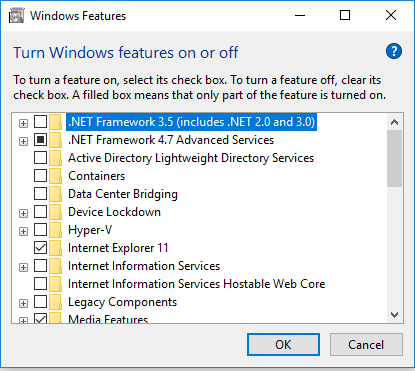
\includegraphics[width=.5 \textwidth]{images/progsycar}
		\caption{Características de Windows.}
		\label{image:car}
\end{figure}
\FloatBarrier

Una vez aquí debemos buscar el Protocolo Simple de Administración de Redes (SNMP) o \textit{Simple Network Management Protocol (SNMP)} y activar su casilla correspondiente así como la de del nodo que se origina a partir de él tal y como se indica en la \ref{image:snmpcar}.

\FloatBarrier
\begin{figure}[htbp!]
		\centering
			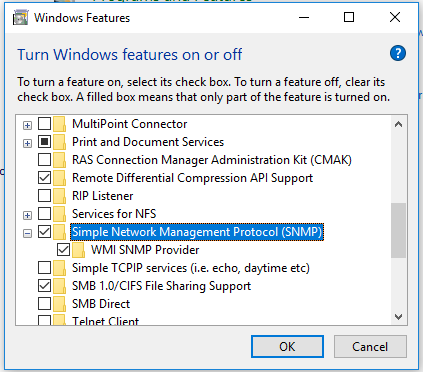
\includegraphics[width=.5 \textwidth]{images/snmpCar}
		\caption{Protocolo SNMP.}
		\label{image:snmpcar}
\end{figure}
\FloatBarrier

El siguiente paso será iniciar el servicio de SNMP y de captura SNMP. Para ello entramos a los \textbf{Servicios} de Windows y buscamos \textbf{Captura SNMP} o \textbf{\textit{SNMP Trap}} como se indica en la figura \ref{image:startSNMPtrap}. Hacemos clic derecho sobre él y lo iniciamos:

\FloatBarrier
\begin{figure}[htbp!]
		\centering
			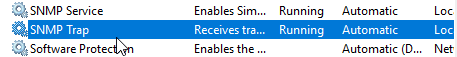
\includegraphics[width=.5 \textwidth]{images/startSNMPtrap}
		\caption{Captura SNMP.}
		\label{image:startSNMPtrap}
\end{figure}
\FloatBarrier

Después, buscamos el servicio \textbf{SNMP} o \textbf{\textit{SNMP Service}}, hacemos clic derecho sobre él y en la pestaña de \textbf{Capturas} o \textbf{Traps} ingresamos el nombre de la comunidad a la que pertenecerá el agente como se observa en la figura \ref{image:comunidad}.

\FloatBarrier
\begin{figure}[htbp!]
		\centering
			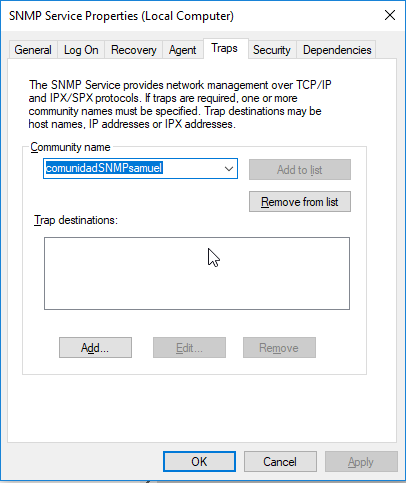
\includegraphics[width=.4 \textwidth]{images/comunidad}
		\caption{Comunidad SNMP.}
		\label{image:comunidad}
\end{figure}
\FloatBarrier

Posteriormente, como observamos en la figura \ref{image:permisos}, debemos establecer los permisos que tendrá la comunidad anterior sobre el agente. Para ello, nos dirigimos a la pestaña de \textbf{Seguridad} o \textbf{Security}, hacemos clic en \textbf{Agregar} o \textbf{Add} y establecemos los permisos de \textbf{Lectura y Escritura} o \textbf{Read and Write}.

\FloatBarrier
\begin{figure}[htbp!]
		\centering
			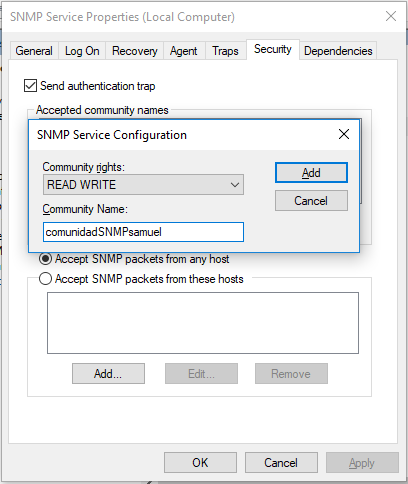
\includegraphics[width=.4 \textwidth]{images/permisos}
		\caption{Permisos de la comunidad.}
		\label{image:permisos}
\end{figure}
\FloatBarrier

Finalmente, escribimos el nombre de la comunidad, tal y como se observa en la figura \ref{image:paquetes}; y habilitamos la opción de \textbf{Aceptar paquetes de cualquier host}. Hacemos clic en \textbf{Aplicar}, \textbf{Aceptar} y reiniciamos el servicio de SNMP.

\FloatBarrier
\begin{figure}[htbp!]
		\centering
			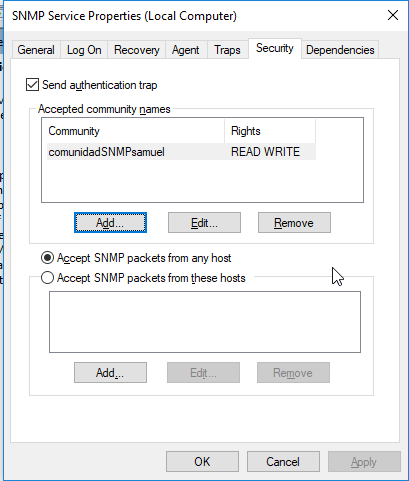
\includegraphics[width=.4 \textwidth]{images/paquetes}
		\caption{Servicio SNMP.}
		\label{image:paquetes}
\end{figure}
\FloatBarrier

Como paso adicional, se deben agregar las reglas de firewall de Windows que permitan la transmisión y recepción de paquetes SNMP. Sin embargo, para este caso de prueba procederemos a desactivar completamente el firewall de Windows. En este caso, al ser una versión de Windows 10 nos dirigimos a \textbf{Windows Defender} y lo deshabilitamos:

\FloatBarrier
\begin{figure}[htbp!]
		\centering
			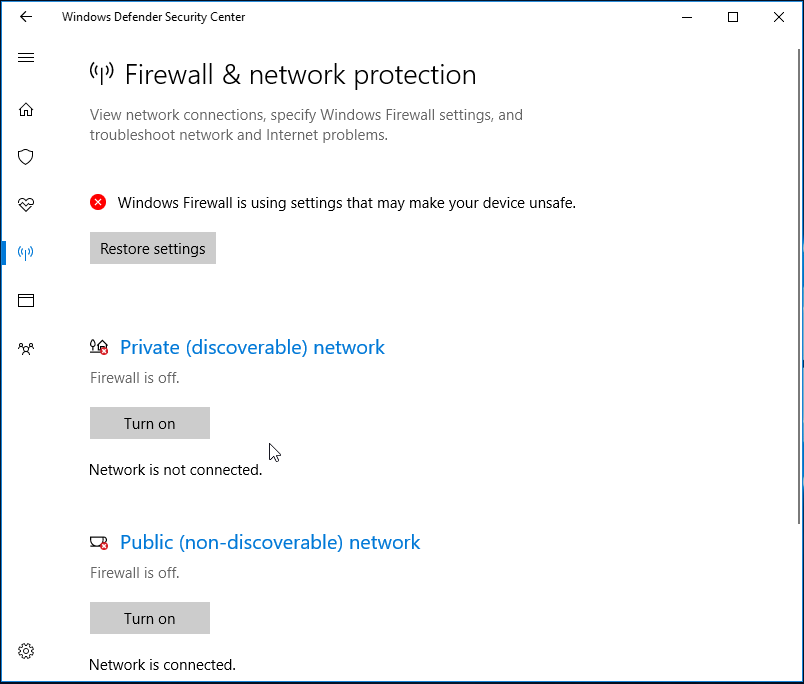
\includegraphics[width=.7 \textwidth]{images/firewall}
		\caption{Firewall de Windows.}
		\label{image:firewall}
\end{figure}
\FloatBarrier